\documentclass[aspectratio=169]{beamer}
\usetheme{Madrid}
\usecolortheme{default}

% Packages
\usepackage{graphicx}
\usepackage{booktabs}
\usepackage{tikz}
% \usepackage{enumitem} % REMOVED: This package conflicts with Beamer and causes the "TeX capacity exceeded" crash.
\usepackage{hyperref}

% Title Information
\title{Arabic RAG Query Enhancement}
\subtitle{Progress Report \& Methodology Finalization}
\author{Mohammed Elhaj \and Osman Bashir}
\institute{Department of Electrical and Electronic Engineering\\Faculty of Engineering\\University of Khartoum}
\date{January 2, 2026}

\begin{document}

% Title Slide
\begin{frame}
\titlepage
\end{frame}

% Table of Contents
\begin{frame}{Agenda}
\tableofcontents
\end{frame}

% ============================================
% SECTION 1: PROJECT OVERVIEW
% ============================================
\section{Project Overview}

\begin{frame}{Project Title \& Objective}
\textbf{Title:} Improving Retrieval Recall in Arabic RAG Systems via Query Enhancement

\vspace{0.5cm}

\textbf{Core Hypothesis:}
\begin{itemize}
    \item Standard retrieval fails in Arabic due to \textbf{morphological \& dialectal gaps}
    \item Query enhancement can bridge this gap before retrieval
    \item Improved queries → Better retrieval → Better RAG performance
\end{itemize}

\vspace{0.5cm}

\textbf{Research Question:}\\
\textit{Can query enhancement techniques improve retrieval recall for Arabic RAG systems, and which techniques are most effective?}
\end{frame}

\begin{frame}{Project Evolution: The Pivot}
\begin{columns}
\column{0.48\textwidth}
\textbf{Original Scope (Oct-Nov 2025):}
\begin{itemize}
    \item Broad RAG enhancement
    \item GraphRAG exploration
    \item Agentic workflows
    \item Multiple components
\end{itemize}

\vspace{0.3cm}
\textcolor{red}{\textbf{Challenge:}} Too complex, multiple variables, unclear contribution

\column{0.48\textwidth}
\textbf{Current Scope (Jan 2026):}
\begin{itemize}
    \item \textbf{Focused:} Query Enhancement only
    \item Simple baseline RAG
    \item Modular approach
    \item Clear evaluation
\end{itemize}

\vspace{0.3cm}
\textcolor{green}{\textbf{Advantage:}} Manageable, measurable, scalable through experiments
\end{columns}

\vspace{0.5cm}
\textbf{Pivot Rationale:} Based on expert consultation (Mohamed Rashad) and literature analysis
\end{frame}

% ============================================
% SECTION 2: METHODOLOGY
% ============================================
\section{Finalized Methodology}

\begin{frame}{System Architecture}
\begin{center}
% Added align=center to nodes to allow line breaks (\\)
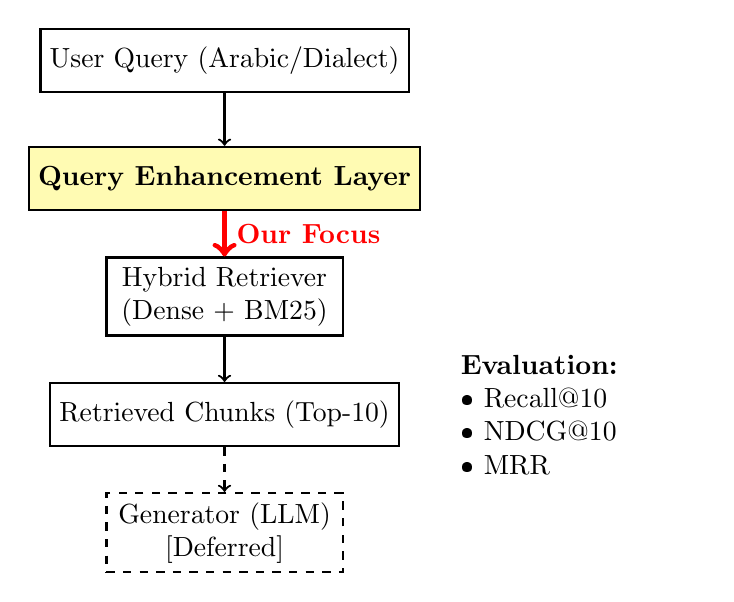
\begin{tikzpicture}[node distance=1.5cm, auto, thick]
    % Nodes
    \node[draw, rectangle, minimum width=3cm, minimum height=0.8cm, align=center] (query) {User Query (Arabic/Dialect)};
    \node[draw, rectangle, minimum width=3cm, minimum height=0.8cm, fill=yellow!30, below of=query, align=center] (enhance) {\textbf{Query Enhancement Layer}};
    \node[draw, rectangle, minimum width=3cm, minimum height=0.8cm, below of=enhance, align=center] (retriever) {Hybrid Retriever\\(Dense + BM25)};
    \node[draw, rectangle, minimum width=3cm, minimum height=0.8cm, below of=retriever, align=center] (chunks) {Retrieved Chunks (Top-10)};
    % Added braces around [Deferred] so it isn't read as a spacing argument for \\
    \node[draw, rectangle, minimum width=3cm, minimum height=0.8cm, below of=chunks, dashed, align=center] (generator) {Generator (LLM)\\{[Deferred]}};
    
    % Arrows
    \draw[->] (query) -- (enhance);
    \draw[->, line width=2pt, red] (enhance) -- node[right] {\textcolor{red}{\textbf{Our Focus}}} (retriever);
    \draw[->] (retriever) -- (chunks);
    \draw[->, dashed] (chunks) -- (generator);
    
    % Annotation
    \node[right of=chunks, node distance=4.5cm, text width=3cm, align=left] (eval) {
        \textbf{Evaluation:}\\
        • Recall@10\\
        • NDCG@10\\
        • MRR
    };
\end{tikzpicture}
\end{center}
\end{frame}

\begin{frame}{Approach: Technology-Oriented}
\textbf{Decision:} Apply techniques first, discover problems they solve

\vspace{0.3cm}

\begin{columns}
\column{0.48\textwidth}
\textbf{Technology-Oriented:}
\begin{itemize}
    \item[+] Safer with existing datasets
    \item[+] Can discover multiple problems
    \item[+] Easier to scale experiments
    \item[+] Aligns with expert advice
\end{itemize}

\column{0.48\textwidth}
\textbf{Problem-Oriented (Alternative):}
\begin{itemize}
    \item[+] Clearer research narrative
    \item[+] Targeted contribution
    \item[-] Requires specific dataset
    \item[-] Riskier if problem ill-defined
\end{itemize}
\end{columns}

\vspace{0.5cm}

\textbf{Current Stance:} Technology-oriented for Checkpoint 1, may refine based on results

\vspace{0.3cm}

\textcolor{blue}{\textbf{Question for Supervisor:}} Do you agree with this approach, or should we pre-define a specific problem (e.g., dialectal mismatch)?
\end{frame}

\begin{frame}{Dataset Selection: MIRACL (Arabic)}
\textbf{Primary Dataset:} MIRACL Arabic subset

\vspace{0.3cm}

\begin{columns}
\column{0.48\textwidth}
\textbf{Why MIRACL?}
\begin{itemize}
    \item Retrieval-focused task
    \item High-quality annotations
    \item Native speaker queries
    \item Natural query-doc mismatch
    \item Gold passages + hard negatives
    \item Industry standard
\end{itemize}

\column{0.48\textwidth}
\textbf{Statistics:}
\begin{itemize}
    \item 2.1M Arabic Wikipedia passages
    \item ~2,896 queries (train/dev/test)
    \item Avg query: 8 words
    \item Avg passage: 100 words
    \item Relevance: 0-3 scale
\end{itemize}
\end{columns}

\vspace{0.5cm}

\textbf{Limitation:} MSA-only (no dialectical coverage)\\
\textbf{Secondary Dataset:} Arabic QA (90K questions, difficulty labels) for generalization
\end{frame}

\begin{frame}{Query Enhancement Techniques (Candidates)}
\begin{enumerate}
    \item \textbf{HyDE (Hypothetical Document Embeddings)}
    \begin{itemize}
        \item Generate hypothetical MSA document from query
        \item Use generated document for retrieval
        \item Works for both dense and sparse retrieval
    \end{itemize}
    
    \item \textbf{Query Rewriting}
    \begin{itemize}
        \item Transform dialect queries → MSA
        \item Normalize morphological variations
        \item LLM-based or rule-based
    \end{itemize}
    
    \item \textbf{Query Expansion}
    \begin{itemize}
        \item Add synonyms, related terms
        \item Handle Arabic morphology (roots, patterns)
    \end{itemize}
    
    \item \textbf{Query Decomposition}
    \begin{itemize}
        \item Break complex queries into sub-queries
        \item Handle multi-hop reasoning
    \end{itemize}
\end{enumerate}

\textbf{First Implementation:} HyDE or Query Rewriting (to be decided after baseline)
\end{frame}

% ============================================
% SECTION 3: PROJECT CHECKPOINTS
% ============================================
\section{Project Roadmap}

\begin{frame}{Checkpoint Strategy}
\begin{center}
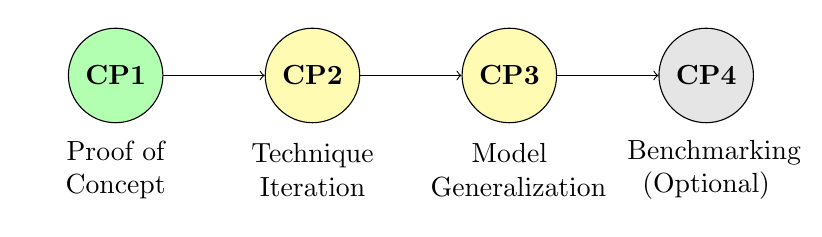
\begin{tikzpicture}[node distance=2.5cm, auto]
    % Checkpoints
    \node[draw, circle, fill=green!30, minimum size=1.2cm] (cp1) {\textbf{CP1}};
    \node[draw, circle, fill=yellow!30, minimum size=1.2cm, right of=cp1] (cp2) {\textbf{CP2}};
    \node[draw, circle, fill=yellow!30, minimum size=1.2cm, right of=cp2] (cp3) {\textbf{CP3}};
    \node[draw, circle, fill=gray!20, minimum size=1.2cm, right of=cp3] (cp4) {\textbf{CP4}};
    
    % Arrows
    \draw[->] (cp1) -- (cp2);
    \draw[->] (cp2) -- (cp3);
    \draw[->] (cp3) -- (cp4);
    
    % Labels
    \node[below of=cp1, node distance=1.2cm, text width=2cm, align=center] {Proof of\\Concept};
    \node[below of=cp2, node distance=1.2cm, text width=2cm, align=center] {Technique\\Iteration};
    \node[below of=cp3, node distance=1.2cm, text width=2cm, align=center] {Model\\Generalization};
    \node[below of=cp4, node distance=1.2cm, text width=2cm, align=center] {Benchmarking\\(Optional)};
\end{tikzpicture}
\end{center}

\vspace{0.5cm}

\textbf{Scalability Strategy:}
\begin{itemize}
    \item Each checkpoint adds a dimension of experiments
    \item Versioning: Arabic HyDE v0.1, v0.2, v0.3...
    \item Contribution grows with each checkpoint completed
\end{itemize}
\end{frame}

\begin{frame}{Checkpoint 1: Proof of Concept (Current Focus)}
\textbf{Goal:} Prove query enhancement improves Arabic RAG retrieval

\vspace{0.3cm}

\textbf{Fixed Variables:}
\begin{itemize}
    \item Single embedding model (BGE-m3, Jina AI, or Qwen - selection in progress)
    \item Single dataset (MIRACL Arabic)
    \item Single query enhancement technique (HyDE or Query Rewriting)
\end{itemize}

\vspace{0.3cm}

\textbf{Success Criteria:}
\begin{itemize}
    \item Measurable improvement in Recall@10, NDCG@10
    \item Clear documentation of what improved and why
    \item Reproducible baseline and enhanced system
\end{itemize}

\vspace{0.3cm}

\textbf{Timeline:} 2-3 weeks

\vspace{0.3cm}

\textbf{Deliverables:}
\begin{itemize}
    \item Baseline performance report
    \item Enhanced system performance report
    \item Comparative analysis
\end{itemize}
\end{frame}

\begin{frame}{Checkpoints 2-4: Scaling Strategy}
\textbf{Checkpoint 2: Technique Iteration}
\begin{itemize}
    \item Test multiple query enhancement approaches
    \item Version and compare (HyDE v0.1, v0.2, Query Rewriting, Expansion...)
    \item Identify best-performing configurations
\end{itemize}

\vspace{0.3cm}

\textbf{Checkpoint 3: Model Generalization}
\begin{itemize}
    \item Test across different embedding models
    \item Validate technique-model compatibility
    \item Test on secondary dataset (Arabic QA)
\end{itemize}

\vspace{0.3cm}

\textbf{Checkpoint 4: Benchmarking (Optional)}
\begin{itemize}
    \item Compare with other RAG systems
    \item Evaluate generation impact (F1, Exact Match)
    \item Test on English datasets (prove language-agnostic)
\end{itemize}

\vspace{0.3cm}

\textit{Note: Checkpoints 2-4 depend on time available and Checkpoint 1 results}
\end{frame}

% ============================================
% SECTION 4: PROGRESS UPDATE
% ============================================
\section{Progress Update}

\begin{frame}{What We've Accomplished}
\textbf{Literature Review (Oct-Dec 2025):}
\begin{itemize}
    \item Analyzed 15+ papers on RAG, query enhancement, and Arabic NLP
    \item Identified key techniques: HyDE, RQ-RAG, QE-RAG, LevelRAG
    \item Mapped English techniques to Arabic challenges
\end{itemize}

\vspace{0.3cm}

\textbf{Dataset Analysis (Dec 2025 - Jan 2026):}
\begin{itemize}
    \item Evaluated 10+ Arabic datasets (MIRACL, TyDi QA, ARCD, Arabic QA, etc.)
    \item Generated comprehensive comparison report using Gemini
    \item Selected MIRACL as primary dataset with clear rationale
\end{itemize}

\vspace{0.3cm}

\textbf{Expert Consultation (Jan 2026):}
\begin{itemize}
    \item Consulted with Mohamed Rashad (AI Researcher, Saudi Arabia)
    \item Received feedback on approach: simple baseline + query enhancement
    \item Validated checkpoint strategy and scalability plan
\end{itemize}

\vspace{0.3cm}

\textbf{Methodology Finalization (Jan 2, 2026):}
\begin{itemize}
    \item 4-part planning meeting (full transcription available)
    \item Finalized architecture, dataset, and approach
    \item Documented all decisions and open questions
\end{itemize}
\end{frame}

\begin{frame}{Current Status \& Documentation}
\textbf{Documentation Created:}
\begin{itemize}
    \item \texttt{RESEARCH\_CONTEXT\_KERNEL.md} - Project overview \& status
    \item \texttt{meetings/2.1.2026\_meeting\_outcomes.md} - Complete methodology
    \item \texttt{research\_decisions/technical\_specifications.md} - Architecture details
    \item \texttt{research\_decisions/open\_questions.md} - Pending decisions
    \item \texttt{meetings/Consultation with Mohammed Rashad.md} - Expert feedback
    \item Chapter 2 draft (Literature Review) - Ready for review
\end{itemize}

\vspace{0.3cm}

\textbf{Current Phase:} Implementation Planning

\vspace{0.3cm}

\textbf{Next Immediate Steps:}
\begin{enumerate}
    \item Finalize embedding model selection (this week)
    \item Download \& preprocess MIRACL dataset
    \item Implement baseline RAG system
    \item Establish evaluation pipeline
\end{enumerate}
\end{frame}

% ============================================
% SECTION 5: CHALLENGES & QUESTIONS
% ============================================
\section{Challenges \& Open Questions}

\begin{frame}{Key Challenges}
\begin{enumerate}
    \item \textbf{Dialectical Gap}
    \begin{itemize}
        \item MIRACL is MSA-only
        \item Real-world queries often dialectal
        \item \textit{Mitigation:} Defer to Checkpoint 2 or use secondary dataset
    \end{itemize}
    
    \item \textbf{Evaluation Granularity}
    \begin{itemize}
        \item Need to understand \textit{what} improved, not just \textit{that} it improved
        \item \textit{Mitigation:} Error analysis, query categorization, case studies
    \end{itemize}
    
    \item \textbf{Resource Constraints}
    \begin{itemize}
        \item Limited GPU access, API costs, time pressure
        \item \textit{Mitigation:} Use free tiers, prioritize experiments, cache embeddings
    \end{itemize}
    
    \item \textbf{Contribution Clarity}
    \begin{itemize}
        \item Unclear if adapting techniques or solving problems
        \item \textit{Mitigation:} Clarify after Checkpoint 1 results
    \end{itemize}
\end{enumerate}
\end{frame}

\begin{frame}{Questions for Supervisor}
\begin{enumerate}
    \item \textbf{Approach Validation:}\\
    Do you agree with the technology-oriented approach, or should we pre-define a specific problem (e.g., dialectal mismatch)?
    
    \vspace{0.3cm}
    
    \item \textbf{Scope Confirmation:}\\
    Is focusing on retrieval metrics (not generation) acceptable for the graduation project?
    
    \vspace{0.3cm}
    
    \item \textbf{Dialectical Priority:}\\
    Should we prioritize dialectical support in Checkpoint 1, or defer it to later stages?
    
    \vspace{0.3cm}
    
    \item \textbf{Contribution Expectations:}\\
    What level of contribution is expected? Technique adaptation vs. novel method?
    
    \vspace{0.3cm}
    
    \item \textbf{Timeline \& Milestones:}\\
    What are the key deadlines and expected deliverables for the graduation project?
    
    \vspace{0.3cm}
    
    \item \textbf{Resources \& Support:}\\
    Any recommendations for computational resources or potential collaborations?
\end{enumerate}
\end{frame}

% ============================================
% SECTION 6: TIMELINE
% ============================================
\section{Timeline \& Next Steps}

\begin{frame}{Project Timeline}
\begin{table}
\small
\begin{tabular}{lll}
\toprule
\textbf{Phase} & \textbf{Duration} & \textbf{Key Deliverables} \\
\midrule
Literature Review & Oct-Dec 2025 & Paper summaries, gap analysis \\
Dataset Analysis & Dec 2025 - Jan 2026 & Dataset selection report \\
\textcolor{green}{\textbf{Baseline Setup}} & \textcolor{green}{\textbf{Jan 2026 (Weeks 1-2)}} & \textcolor{green}{\textbf{Baseline system, metrics}} \\
Query Enhancement & Jan-Feb 2026 (Weeks 3-4) & Enhanced system, experiments \\
Analysis \& Iteration & Feb 2026 (Weeks 5-6) & Results analysis, refinement \\
Generalization & Feb-Mar 2026 (Optional) & Multi-model, multi-dataset tests \\
Thesis Writing & Mar-Apr 2026 & Complete thesis draft \\
Final Review & Apr-May 2026 & Thesis submission \\
\bottomrule
\end{tabular}
\end{table}

\vspace{0.3cm}

\textbf{Current Focus:} Baseline Setup (Weeks 1-2)

\vspace{0.3cm}

\textit{Note: Timeline is flexible and will be adjusted based on supervisor feedback and progress}
\end{frame}

\begin{frame}{Immediate Next Steps (This Week)}
\begin{enumerate}
    \item \textbf{Embedding Model Selection}
    \begin{itemize}
        \item Review MIRACL leaderboard
        \item Test BGE-m3, Jina AI, Qwen on sample queries
        \item Measure Recall@10, inference time, cost
        \item \textbf{Decision by:} End of this week
    \end{itemize}
    
    \item \textbf{MIRACL Dataset Setup}
    \begin{itemize}
        \item Download Arabic Wikipedia dumps
        \item Preprocess and chunk passages
        \item Load queries and relevance judgments
        \item Set up data loaders
    \end{itemize}
    
    \item \textbf{Baseline Implementation}
    \begin{itemize}
        \item Implement dense retrieval (selected embedding model)
        \item Implement sparse retrieval (BM25)
        \item Implement hybrid retrieval
        \item Establish evaluation pipeline
    \end{itemize}
    
    \item \textbf{Documentation}
    \begin{itemize}
        \item Update research context with supervisor feedback
        \item Document baseline implementation
        \item Prepare for Checkpoint 1 experiments
    \end{itemize}
\end{enumerate}
\end{frame}

% ============================================
% FINAL SLIDE
% ============================================
\begin{frame}{Summary}
\textbf{Project Status:} Methodology finalized, ready for implementation

\vspace{0.3cm}

\textbf{Key Decisions:}
\begin{itemize}
    \item Focus: Query Enhancement for Arabic RAG
    \item Dataset: MIRACL (Arabic subset)
    \item Approach: Technology-oriented with checkpoint strategy
    \item Architecture: Simple baseline + query enhancement layer
\end{itemize}

\vspace{0.3cm}

\textbf{Strengths:}
\begin{itemize}
    \item Clear, focused scope
    \item Scalable through experiments
    \item Strong theoretical foundation
    \item Expert-validated approach
\end{itemize}

\vspace{0.3cm}

\textbf{Next Milestone:} Checkpoint 1 completion (2-3 weeks)

\vspace{0.5cm}

\begin{center}
\Large{\textbf{Thank you!}}\\
\vspace{0.3cm}
\normalsize{Questions \& Discussion}
\end{center}
\end{frame}

\end{document}